
%%%%%%%%%%%%%%%%%%%%%%%%%%%%%%%%%%%%%%%%%%%%%%%%%%%%%%%%%%%%%%%%%%%%%%%%%%%%%%%%%%%%%%%%
%%%%%%%%%%%%%%%%% Keyfitz's entropy threshold age %%%%%%%%%%%%%%%%%%%%%%%
%%%%%%%%%%%%%%%%%%%%%%%%%%%%%%%%%%%%%%%%%%%%%%%%%%%%%%%%%%%%%%%%%%%%%%%%%%%%%%%%%%%%%%%%

\documentclass[a4paper,twoside, openright, 12pt, leqno]{article}

% Upload template for articles
% \usepackage{ArticleTemp}

\usepackage[top=3.5cm, bottom=2.5cm, outer=2.5cm, inner=2.5cm, headsep=1.5cm, footskip=1.2cm, headheight=14pt]{geometry}
\usepackage{amsmath}
\usepackage{amsthm}                             % Proof environment
\usepackage{amssymb}
\usepackage{enumitem}				% Different enumarate options
\usepackage{graphicx}				% standard LaTeX graphics tool
\usepackage{natbib}				% Bibliography
\usepackage{setspace}				% Control line space
\usepackage{afterpage}				% Control the subsequent page
\usepackage[bottom]{footmisc}			% Manage footnotes. Used to modify the indentation and force footnotes bottom page. Necessary befor hyperref !!!
\usepackage{etoolbox}				% Add patches
\usepackage{url}				% Include URL in the references
\usepackage[width=0.95\textwidth]{caption} 	% Mange font size and margins of captions
\usepackage{changepage}				% Temporary change page settings
\usepackage[rightmargin=0em]{quoting}		% Add quotations in text
\usepackage{multirow}				% Multiple rows in tables
\usepackage{placeins}				% Use \FloatBarrier to put figures and tables in current section
\usepackage{booktabs}
 \usepackage[hyperfootnotes=false, colorlinks = true, allcolors = blue]{hyperref}		% Include hyperlinks
\usepackage{fancyhdr}				% Fancy headers


% Hyperlinks in references only for YEAR
\makeatletter
% Patch case where name and year are separated by aysep
\patchcmd{\NAT@citex}
{\@citea\NAT@hyper@{%
		\NAT@nmfmt{\NAT@nm}%
		\hyper@natlinkbreak{\NAT@aysep\NAT@spacechar}{\@citeb\@extra@b@citeb}%
		\NAT@date}}
{\@citea\NAT@nmfmt{\NAT@nm}%
	\NAT@aysep\NAT@spacechar\NAT@hyper@{\NAT@date}}{}{}
% Patch case where name and year are separated by opening bracket
\patchcmd{\NAT@citex}
{\@citea\NAT@hyper@{%
		\NAT@nmfmt{\NAT@nm}%
		\hyper@natlinkbreak{\NAT@spacechar\NAT@@open\if*#1*\else#1\NAT@spacechar\fi}%
		{\@citeb\@extra@b@citeb}%
		\NAT@date}}
{\@citea\NAT@nmfmt{\NAT@nm}%
	\NAT@spacechar\NAT@@open\if*#1*\else#1\NAT@spacechar\fi\NAT@hyper@{\NAT@date}}
{}{}
\makeatother

% Customize headers
\pagestyle{fancy}
\fancyhf{}
\fancyhead[RO,LE]{\small\thepage}
\fancyhead[LO]{\small \nouppercase{The threshold age of the lifetable entropy}}
\fancyhead[RE]{\small \nouppercase{Aburto et al.}}
\fancyfoot[L,R,C]{}
\renewcommand{\headrulewidth}{0.4pt}


% TABLES: Alignment columns	
\usepackage{array}
\newcolumntype{L}[1]{>{\raggedright\let\newline\\\arraybackslash\hspace{0pt}}m{#1}}
\newcolumntype{C}[1]{>{\centering\let\newline\\\arraybackslash\hspace{0pt}}m{#1}}
\newcolumntype{R}[1]{>{\raggedleft\let\newline\\\arraybackslash\hspace{0pt}}m{#1}}

% Clear page in some cases at the end of section
\newcommand*{\stopsection}{%
  \par
  \vspace{\fill}%
  \pagebreak[0]%
  \vspace{-\fill}%
}

% New command \xbar to make bar wider
\newcommand*\xbar[1]{%
   \hbox{%
     \vbox{%
       \hrule height 0.5pt % The actual bar
       \kern0.3ex%         % Distance between bar and symbol
       \hbox{%
         \kern-0.28em%      % Shortening on the left side
         \ensuremath{#1}%
         \kern-0.05em%      % Shortening on the right side
       }%
     }%
   }%
} 

% Proposition for the Appendix
\newtheorem{theorem}{Proposition}

% Numbering subsubsections
\setcounter{secnumdepth}{3}

% References with no comma
\setcitestyle{aysep={}}	

% Footnote indentation
\setlength{\footnotemargin}{0.6em}

% Distance between footnote number and text
\renewcommand{\footnotelayout}{\hspace{0.28em}}

% Delete page number
\pagenumbering{gobble}

% Comma to separate footnotes
\newcommand\fnsep{\textsuperscript{,}}

% % One footnote with asterisk
 % \renewcommand{\thefootnote}{\fnsymbol{footnote}}
 \newcommand{\astfootnote}[1]{
 % \let\oldthefootnote=\thefootnote
 \setcounter{footnote}{0}
 \renewcommand{\thefootnote}{\fnsymbol{footnote}}
 \footnote{#1}
 % \let\thefootnote=\oldthefootnote
 \setcounter{footnote}{0}
 }

% Allow customizing symbol in selected footnotes
\makeatletter
\def\@xfootnote[#1]{%
  \protected@xdef\@thefnmark{#1}%
  \@footnotemark\@footnotetext}
\makeatother



%%%%%%%%%%%%%%%%%%%%%%%%%%%%%%%%%%%%%%%%%%%%%%%%%%%%%%%%%%%%%%%%%%%%%%%%%%%%%%%%%%%%%%%%
%%%%%%%%%%%%%%%%%%%%%%%%%%%%%%%%%%%%%%%%%%%%%%%%%%%%%%%%%%%%%%%%%%%%%%%%%%%%%%%%%%%%%%%%

% Begin document
\begin{document}

% Affilations as footnotes with symmbols
\renewcommand{\thefootnote}{\alph{footnote}}

% Remove header from the first page
\thispagestyle{empty}

\begin{center}
    
    \vspace*{1cm}
    \LARGE{The threshold age of the lifetable entropy}	
    \vspace{.4cm}    
        
    % \hypersetup{footnotecolor=black}
           
    \vspace{1cm}
    \large Jos\'e Manuel Aburto\footnote[*]{Correspondence:~\href{mailto:jmaburto@sdu.dk}{jmaburto@sdu.dk}.}\footnote{Interdisciplinary Center on Population Dynamics, University of Southern Denmark, Odense, Denmark.}\fnsep\footnote{Max Planck Institute for Demographic Research, Rostock, Germany.}, Jesus-Adrian Alvarez\textsuperscript{a}, Francisco Villavicencio\footnote{Institute for International Programs, Bloomberg School of Public Health, Johns Hopkins University, Baltimore, MD, United States.}\fnsep\textsuperscript{a}\\ and James W. Vaupel\textsuperscript{a}\fnsep\textsuperscript{b}
    
    \vspace{1cm}
    \large\today
    \vspace{1cm}
       
\end{center}

% In text use numbers for footnotes
\renewcommand{\thefootnote}{\arabic{footnote}}
\setcounter{footnote}{0}


\section*{Abstract}
\bigskip

\textbf{BACKGROUND} \\
Indicators of relative variation of lifespans are important because they capture the dimensionless shape of aging. They are markers of inequality at the population level and express the uncertainty at the time of death at the individual level. In particular, the lifetable entropy $\,\xbar{H}$ represents the elasticity of life expectancy to a change in mortality and it has been used as an indicator of lifespan variation. However, it is unknown how this measure changes over time and whether a threshold age exists, as it does for other lifespan variation indicators.
\bigskip

\noindent\textbf{RESULTS} \\
The time derivative of $\,\xbar{H}$ can be decomposed into changes in life disparity $e^\dagger$ and life expectancy at birth $e_o$. Likewise, changes over time in $\,\xbar{H}$ are a weighted average of age-specific rates of mortality improvements. These weights reflect the sensitivity of $\,\xbar{H}$ and show how mortality improvements can increase (or decrease) the relative inequality of lifespans. Further, we prove that in the assumption that mortality is reduced at all ages, $\,\xbar{H}$, as well as $e^\dagger$, has a threshold age below which saving lives reduces entropy, whereas improvements above that age increase entropy.
\bigskip

\noindent\textbf{CONTRIBUTION} \\
We give a formal expression for changes over time of $\,\xbar{H}$, and provide a formal proof of the existence of a unique threshold age that separates reductions and increases in lifespan variation as a result age-specific mortality improvements.

% Line interpsace
\linespread{2}\normalsize
\clearpage


%%%%%%%%%%%%%%%%%%%%%%%%%%%%%%%%%%%%%%%%%%%%%%%%%%%%%%%%%%%%%%%%%%%%%%%%%%%%%%%%%%%%%%%%
%%%%%%%%%%%%%%%%%%%%%%%%%%%%%%%%%%%%%%%%%%%%%%%%%%%%%%%%%%%%%%%%%%%%%%%%%%%%%%%%%%%%%%%% 

\section{Relationship}
The lifetable entropy is a dimensionless indicator of the relative variation in the length of life compared to life expectancy at birth \citep{keyfitz1968introduction,demetrius1974demographic,Keyfitz1977, demetrius1978adaptive}. It is usually defined as
%
\begin{equation*}
\xbar{H}(t)=-\frac{\int_0^\infty\ell(a, t)\,\ln\ell(a, t)\,da}{\int_0^\infty\ell(a, t)\,da}=\int_0^\infty c(a, t)\,H(a,t)\,da=\frac{e^\dagger(t)}{e_o(t)}\;,
% \label{eq:entropy}
\end{equation*}
%
where $e^\dagger(t)=-\int_0^\infty\ell(a,t)\,\ln\ell(a,t)\,da$ is the life disparity or number of life-years lost as a result of death \citep{Vaupel2003}, $e_o(t)=\int_0^\infty\ell(a, t)\,da$ is the life expectancy at birth at time $t$, $\ell(a,t)$ is the lifetable survival function, $c(a,t)=\ell(a,t)\,/\,\int_0^\infty\ell(x,t)\,dx$ is the population structure, and $H(a,t)=\int_0^a\mu(x,t)\,dx$ is the cumulative hazard to age $a$, where $\mu(x,t)$ is the force of mortality (hazard rate or risk of death) at age $x$ at time $t$. Note that $\,\xbar{H}(t)$ can be interpreted as an \emph{average value} of $H(a,t)$ in the population at time $t$.

\cite{Goldman1986} and \cite{Vaupel1986} proved that
%
$$
e^\dagger(t)=\int_0^\infty d(a, t)\,e(a, t)\,da\;,
$$
%
where $d(a,t)$ represents the distribution of deaths and $e(a,t)=\int_a^\infty\ell(x,t)\,dx\,/\,\ell(a,t)$ the remaining life expectancy at age $a$ at time $t$. This provides an alternative expression for the lifetable entropy as
%
$$
\xbar{H}(t)=\frac{\int_0^\infty d(a, t)\,e(a, t)\,da}{\int_0^\infty\ell(a, t)\,da}\;.
$$

Let $\,\dot{\xbar{H}}$ denote the partial derivative of $\,\xbar{H}$ with respect to time.\footnote{In the following, a dot over a function will denote its partial derivative with respect to time $t$, but variable $t$ will be omitted for simplicity.} We define $\rho(x)=-\dot{\mu}(x)\,/\,\mu(x)$ as the age-specific rates of mortality improvements. Then, the relative derivative of $\,\xbar{H}$ can be expressed as a weighted average of age-specific rates of mortality improvement, 
%
\begin{equation}
\dot{\xbar{H}}\,/\,\,\xbar{H} = \int_0^\infty\rho(x)\,w(x)\,W(x)\,dx\;,
\label{eq:1}
\end{equation}
%
with weights
%
$$
w(x)=\mu(x)\,\ell(x)\,e(x)\qquad\text{and}\qquad W(x)=\frac{1}{e^\dagger}\,\big(H(x)+\,\xbar{H}(x)-1\big)-\frac{1}{e_o}\;.
$$

Function $\,\xbar{H}(x)$ is the lifetable entropy conditioned on surviving to age $x$, defined as
%%
$$
\xbar{H}(x)=\frac{e^\dagger(x)}{e(x)}=\frac{\int_x^\infty d(a)\,e(a)\,da}{\int_x^\infty\ell(a)\,da}\,.
$$
%
where $e^\dagger(x)=\int_x^\infty d(a)\,e(a)\,da\,/\,\ell(x)$ refers to life disparity above age $x$, and $e(x)$ is the remaining life expectancy at age $x$.

Note that the lifetable entropy $\,\xbar{H}$ is a measure of relative lifespan variation. Thus, higher values represent more variation, whereas lower values denote less variation of lifespans. If mortality improvements at all ages occur over time, there exists a unique threshold age $a^H$ that separates \emph{positive} from \emph{negative} contributions to the lifetable entropy $\,\xbar{H}$ resulting from those mortality improvements. This threshold age $a^H$ is reached when
%
\begin{equation}
  H\left(a^H\right)+\,\xbar{H}\left(a^H\right) =1 +\,\xbar{H}\;.
  \label{threhsold.age}
\end{equation}


%%%%%%%%%%%%%%%%%%%%%%%%%%%%%%%%%%%%%%%%%%%%%%%%%%%%%%%%%%%%%%%%%%%%%%%%%%%%%%%%%%%%%%%%
%%%%%%%%%%%%%%%%%%%%%%%%%%%%%%%%%%%%%%%%%%%%%%%%%%%%%%%%%%%%%%%%%%%%%%%%%%%%%%%%%%%%%%%%

\section{Proof}

\cite{Fernandez2015} showed that the relative derivative of $\,\xbar{H}$ can be expressed as
%
\begin{equation}
\dot{\xbar{H}}\,/\,\,\xbar{H}=\frac{\dot{e}^\dagger}{e^\dagger}-\frac{\dot{e}_o}{e_o}\;,
\label{eq:alternative}
\end{equation}
%
This formula indicates that relative changes in $\,\xbar{H}$ over time are given by the difference between relative changes in $e^\dagger$ (dispersion component) and relative changes in $e_o$ (translation component). We will first provide expressions for $\dot{e}_o$ and $\dot{e}^\dagger$ to prove that~\eqref{eq:1} and~\eqref{eq:alternative} are equivalent. Next, we will prove the existence of threshold age for $\,\xbar{H}$ and its uniqueness.

 
\subsection{Relative changes over time in $\,\xbar{H}$}

\cite{Vaupel2003} showed that changes over time in life expectancy at birth are a weighted average of the total rates of mortality improvements, given by
%
\begin{equation}
\label{ex.derivative}
\dot{e}_o=\int_0^\infty\rho(x)\,w(x)\,dx\;,
\end{equation}
%.
where $\rho(x)=-\dot{\mu}(x)\,/\,\mu(x)$ are the age-specific rates of mortality improvement, and $w(x)=\mu(x)\,\ell(x)\,e(x) = d(x)\,e(x)$ is a measure of the importance of death at age $x$. 

Since $d(x)=\mu(x)\,\ell(x)$ and $\ell(x)\,e(x)=\int_x^\infty\ell(a)\,da$, the partial derivative with respect to time of $e^\dagger=\int_0^\infty d(x)\,e(x)\,dx$ can be expressed as
%
\begin{equation*}
 \begin{split}
 \dot{e}^\dagger	& = \int_0^\infty\dot{\mu}(x)\,\ell(x)\,e(x)\,dx+\int_0^\infty\mu(x)\int_x^\infty\dot{\ell}(a)\,da\,dx		\\
			& = -\int_0^\infty\rho(x)\,w(x)\,dx+\int_0^\infty\dot{\ell}(a)\int_0^a\mu(x)\,dx\,da                         \\
			& = -\int_0^\infty\rho(x)\,w(x)\,dx-\int_0^\infty\int_0^a\dot{\mu}(x)\,dx\,\ell(a)\,H(a)\,da\;,
 \end{split}
\end{equation*}
%
where $H(a)$ is the cumulative hazard to age $a$. By reversing the order of integration and doing some additional manipulations, we get

\begin{equation}
 \begin{split}
 \dot{e}^\dagger	
    & = -\int_0^\infty\rho(x)\,w(x)\,dx-\int_0^\infty\dot{\mu}(x)\int_x^\infty\,\ell(a)\,H(a)\,da\,dx    \\
    & = -\int_0^\infty\rho(x)\,w(x)\,dx+\int_0^\infty\rho(x)\,w(x)\,\frac{\int_x^\infty\,\ell(a)\,H(a)\,da}{\ell(x)\,e(x)}\,dx                                   \\
    & =\int_0^\infty\rho(x)\,w(x)\left(\frac{\int_x^\infty\,\ell(a)\big(H(a)-H(x)+H(x)\big)\,da}{\ell(x)\,e(x)}-1\right)dx                  \\
    & =\int_0^\infty\rho(x)\,w(x)\left(H(x)\,\frac{\int_x^\infty\,\ell(a)\,da}{\ell(x)\,e(x)}+\frac{\int_x^\infty\,\ell(a)\big(H(a)-H(x)\big)\,da}{\ell(x)\,e(x)}-1\right)\,dx                                           \\
    & =\int_0^\infty\rho(x)\,w(x)\left(H(x)+\frac{\int_x^\infty\,\ell(a)\big(H(a)-H(x)\big)\,da}{\ell(x)\,e(x)}-1\right)\,dx\;.
 \label{der.edagger}
 \end{split}
\end{equation}

In Proposition~\ref{prop1} in the Appendix, we prove that
%
\begin{equation}
e^\dagger(x)=\frac{1}{\ell(x)}\int_x^\infty d(a)\,e(a)\,da=\frac{1}{\ell(x)}\int_x^\infty\,\ell(a)\big(H(a)-H(x)\big)\,da\;.
\label{eq:edaggerNew}
\end{equation}
%
Replacing~\eqref{eq:edaggerNew} into~\eqref{der.edagger} yields
%
\begin{equation}
  \begin{split}
    \dot{e}^\dagger
        & = \int_0^\infty\rho(x)\,w(x)\left(H(x)+\frac{e^\dagger(x)}{e(x)}-1\right)dx                 \\
        & = \int_0^\infty\rho(x)\,w(x)\,\big(H(x)+\,\xbar{H}(x)-1\big)\,dx   \;.
  \end{split}
  \label{der3.edagger}
\end{equation}
%
Finally, replacing the expressions of $\dot{e}_o$ and $\dot{e}^\dagger$ from~\eqref{ex.derivative} and~\eqref{der3.edagger} into~\eqref{eq:alternative}, we get 
%
\begin{equation*}
 \begin{split}
    \dot{\xbar{H}}\,/\,\,\xbar{H}
        & = \frac{1}{e^\dagger}\int_0^\infty\rho(x)\,w(x)\left(H(x)+\,\xbar{H}(x)-1\right)dx-\frac{1}{e_o}\int_0^\infty\rho(x)\,w(x)\,dx    \\
        & = \int_0^\infty\rho(x)\,w(x)\left(\frac{1}{e^\dagger}\left(H(x)+\,\xbar{H}(x)-1\right)-\frac{1}{e_o}\right)dx                               \\
        & = \int_0^\infty\rho(x)\,w(x)\,W(x)\,dx\;,
 \end{split}
\end{equation*}
%
which proves~\eqref{eq:1} and shows that relative changes over time in the lifetable entropy are the average of the rates of mortality improvement weighted by the product $w(x)\,W(x)$.\hfill$\square$


\subsection{The threshold age for $\,\xbar{H}$}

Using~\eqref{eq:1}, changes over time in the lifetable entropy $\,\xbar{H}$ are given by
%
\begin{equation}
  \dot{\xbar{H}}=\,\xbar{H}\,\int_0^\infty\rho(x)\,w(x)\,W(x)\,dx\;.
  \label{eq:Hprime}
\end{equation}
%
Whenever $\,\dot{\xbar{H}}>0$, lifespan inequality increases over time, whereas $\,\dot{\xbar{H}}<0$ implies that variation of lifespans decreases over time. Because $\ell(x)$ is a positive function bounded between 0 and 1, we have that $\,\xbar{H}>0$. Moreover, assuming age-specific death rates $\mu(x)$ improve over time at all ages, then $\dot{\mu}(x)<0$ and $\rho(x)>0$ at any age $x$. Therefore,~\eqref{eq:Hprime} implies that
%
\begin{enumerate}
  \item Those ages $x$ in which $w(x)\,W(x)>0$ will contribute \emph{positively} to the lifetable entropy $\,\xbar{H}$ and increase lifespan variation;
  \item Those ages $x$ in which $w(x)\,W(x)<0$ will contribute \emph{negatively} to the lifetable entropy $\,\xbar{H}$ and favor lifespan equality;
  \item Those ages $x$ in which $w(x)\,W(x)=0$ will have no effect on the variation over time of $\,\xbar{H}$.
\end{enumerate}
%
Our goal is to prove that if mortality improvements occur for all ages and $\rho(x)>0$, there exists a unique threshold age $a^H$ such that $w\left(a^H\right)\,W\left(a^H\right)=0$. That threshold age will separate \emph{positive} from \emph{negative} contributions to $\,\xbar{H}$ resulting from mortality improvements. 

The product $w(x)\,W(x)$ can be re-expressed as 
%
\begin{equation*}
  \begin{split}
    w(x)\,W(x)	& = \mu(x)\,\ell(x)\,e(x)\,\left(\,\frac{1}{e^\dagger}\left(H(x)+\,\xbar{H}(x)-1\right)-\frac{1}{e_o}\right)	                            \\
                & = \frac{\mu(x)\,\ell(x)\,e(x)}{e^\dagger}\left(H(x)+\,\xbar{H}(x)-\,\xbar{H}-1\right)\;.
  \end{split}
  \label{W_2}
\end{equation*}
%
Since $\mu(x)$, $\ell(x)$, $e(x)$ and $e^\dagger$ are all positive functions, the threshold age of $\,\xbar{H}$ occurs whenever
%
\begin{equation}
\label{g_x}
g(x):= H(x)+\,\xbar{H}(x)-\,\xbar{H}-1=0\;.
\end{equation}

When $x$ is close to 0, $g(x)$ takes negative values since
%
\begin{equation*}
g(0)=H(0)+\,\xbar{H}(0)-\,\xbar{H}-1=0+\,\xbar{H}-\,\xbar{H}-1=-1<0\;.
\end{equation*}
%
Likewise, $g(x)$ takes positive values when $x$ becomes arbitrary large. Note that $\,\xbar{H}$ does not depend on age, and therefore
%
$$
\lim_{x\to\infty}g(x)=\lim_{x\to\infty}\left(H(x)+\,\xbar{H}(x)\right)-\,\xbar{H}-1=\infty
$$
%
because $\lim_{x\to\infty}H(x)=\infty$. By definition, $\,\xbar{H}(x)\geq0$ for all $x$, so regardless of the behavior of $\,\xbar{H}(x)$ when $x$ is arbitrarily large, the limit of $g(x)$ tends to infinity. Hence, given that $g(0)=-1$ and $\lim_{x\to\infty}g(x)=\infty$, in a continuous framework the intermediate value theorem guarantees the existence of at least one age $a^H$ at which $g(a^H)=0$.

Moreover, as shown in Proposition~\ref{prop2} in the Appendix, $g(x)$ is a strictly increasing function, and therefore a one-to-one function assuming continuity. As a result, there is a unique threshold age $a^H$ that separates \emph{positive} from \emph{negative} contributions to the lifetable entropy $\,\xbar{H}$, and that threshold age is reached when
%
\begin{equation*}
w(x)\,W(x)=0\Longleftrightarrow g(x)=0\Longleftrightarrow H(x)+\,\xbar{H}(x)= 1+\,\xbar{H}\;,
\end{equation*}
%
which proves~\eqref{threhsold.age}.\hfill$\square$


%%%%%%%%%%%%%%%%%%%%%%%%%%%%%%%%%%%%%%%%%%%%%%%%%%%%%%%%%%%%%%%%%%%%%%%%%%%%%%%%%%%%%%%%
%%%%%%%%%%%%%%%%%%%%%%%%%%%%%%%%%%%%%%%%%%%%%%%%%%%%%%%%%%%%%%%%%%%%%%%%%%%%%%%%%%%%%%%%

\section{Related results}

Demographers have developed a battery of indicators to measure how lifespans vary in populations \citep{colchero2016emergence,vanRaalte2013}. The most common indexes are the variance \citep{edwards2005inequality, tuljapurkar2011variance}, standard deviation \citep{vanraalte2018Science} and coefficient of variation \citep{aburto2018potential} of the age at death distribution, the Gini coefficient \citep{Shkolnikov2003,archer2018diet, gigliarano2017longevity}, the Theil index \citep{Smits2009}, and the years of life lost \citep{Vaupel2011, Aburto2018Eastern}, among others. However, only few studies have analytically derived formulas for \textit{threshold age} below and above which mortality improvements respectively decrease and increase lifespan variation. \citet{Zhang2009} showed that the threshold age $(a^\dagger)$ for life disparity $(e^\dagger)$ occurs when $H(x)+\,\xbar{H}(x)=1$. Similarly, \citet{Gillespie2014} determined a threshold age for the variance of the age at death distribution. \Citet{vanRaalte2013} also showed that it is possible to determine the threshold age by performing an empirical sensitivity analysis of lifespan variation indicators.

In this article, we contribute to the lifespan variation literature by deriving the threshold age $a^H$ for the lifetable entropy $\,\xbar{H}$. This age separates negative from positive contributions of age-specific mortality improvements. We analytically proved its existence and---in the assumption that mortality improves over time for all ages---also its uniqueness. In Section~\ref{sec:application} we empirically show that it differs from the threshold age of $e^\dagger$.

%%%%%%%%%%%%%%%%%%%%%%%%%%%%%%%%%%%%%%%%%%%%%%%%%%%%%%%%%%%%%%%%%%%%%%%%%%%%%%%%%%%%%%%%
%%%%%%%%%%%%%%%%%%%%%%%%%%%%%%%%%%%%%%%%%%%%%%%%%%%%%%%%%%%%%%%%%%%%%%%%%%%%%%%%%%%%%%%%

\section{Applications}
\label{sec:application}

\subsection{Numerical findings}

Figure~\ref{fig:Fig1} depicts the threshold ages for the two related measures, $e^\dagger$ and $\,\xbar{H}$. Calculations were performed using data from the \citet{HMD} for females in the United States and Italy in 2005. The blue line represents $g(x)$ from Equation~\eqref{g_x}. The threshold age $a^H$ occurs when  $g(x)$ crosses zero. The red and grey line display the same functions that \cite{Zhang2009} used to find the threshold age for $e^\dagger$ rescaled to fit in the graph. The intersection of these two lines denotes the threshold age $a^\dagger$. Finally, the dashed black line depicts the life expectancy at birth. \citet{Vaupel2011} noted that $a^\dagger$ tends to fall just below life expectancy. The threshold age for the lifetable entropy $a^H$ is greater than $a^\dagger$ and is very close above life expectancy for these countries. Note the similarity between the formulas for $a^\dagger$, given by $H(a^\dagger)+\,\xbar{H}(a^\dagger)=1$, and $a^H$, given by $H(a^H)+\,\xbar{H}(a^H)= 1+\,\xbar{H}$.

\begin{figure}[h]
  \centering
  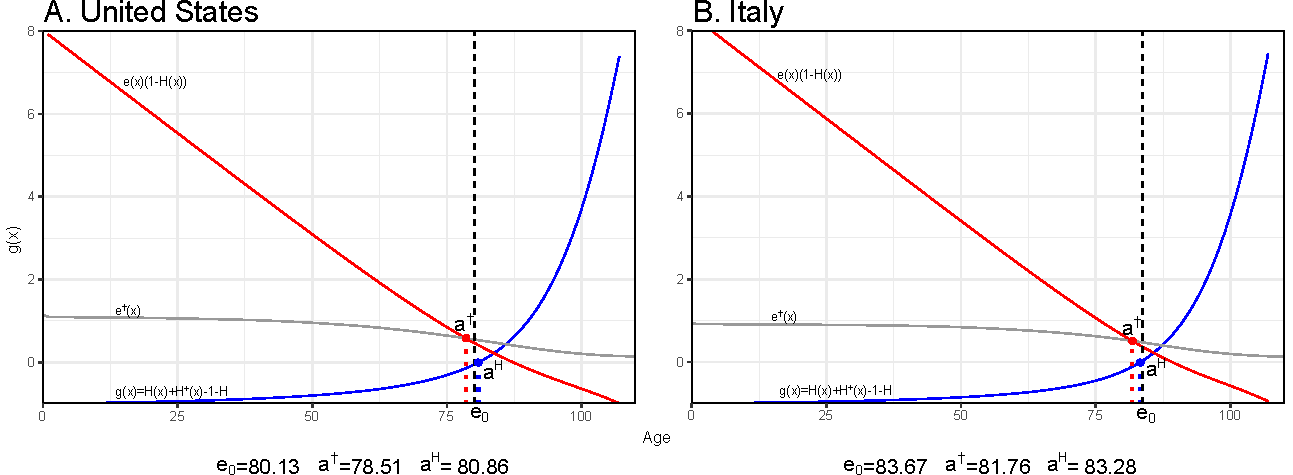
\includegraphics[scale=.72]{Figures/Ages2005}
  \caption{Threshold ages for life disparity $(a^\dagger)$ and for the lifetable entropy $(a^H)$. United States and Italy in 2005. Values in Panel~A: $e_o=80.13$, $a^\dagger=78.51$, and $a^H=80.86$. Values in Panel~B: $e_o=83.67$, $a^\dagger=81.76$, and $a^H=83.28$. Note: functions to determine the threshold age for $e^\dagger$ where rescaled by a factor of 1/10 for comparability. Source: \cite{HMD}.}
  \label{fig:Fig1}
\end{figure}

Panels~A and~B in Figure~\ref{fig:Fig2} illustrate the evolution over time of the threshold ages for $e^\dagger$ and $\,\xbar{H}$ in French and Swedish females, respectively. We chose these countries because they portray large series of reliable data available at the \cite{HMD}. 

Values for $a^\dagger$ are close to life expectancy throughout the period. However, around 1950 there is a crossover between $a^\dagger$ and $e_o$ such that $a^\dagger$ remained close to life expectancy but below it. This result shows that the threshold age $a^\dagger$ being below life expectancy is a modern feature of ageing populations with high life expectancy. From the beginning of the period of observation to the 1950s, the threshold age for the lifetable entropy was above life expectancy for both countries. During some periods $a^\dagger$ was roughly constant whereas life expectancy trended upwards. After the 1950s, $a^H$ converged towards life expectancy. We further analyzed this observation assuming the hazard follows a Gompertz model (see Appendix). Our analysis showed that the threshold age $a^H$ of the lifetable entropy $\,\xbar{H}$ for the Gompertz model is proportional to $e_o$ by a factor $\delta$ that depends on the Gompertz parameters. Moreover, this parameter $\delta$ indicates that the empirical correspondence between the threshold age and life expectancy at birth  comes from the fact that mortality in modern mortality schedules are roughly following a Gompertz model. Therefore, it can be speculated that the difference between the threshold age and life expectancy in earlier years come from the fact that a big proportion of mortality was occurring in ages where the force of mortality does not follow a Gompertz such as in infancy. This is consistent with historical patterns which suggest that, since hunter-gathers to modern populations, death rates have decreased at all ages but mostly at young ages \citep{burger2012human}. The code and data to reproduce these results are publicly available through the repository in the link \url{https://bit.ly/2wqzOFp}.

\begin{figure}[h]
  \centering
  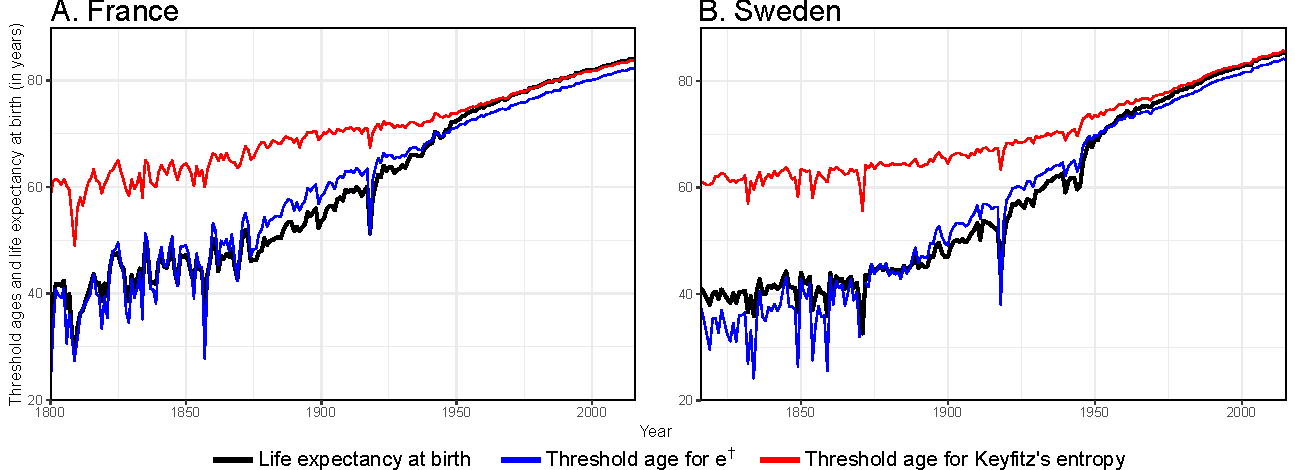
\includegraphics[scale=.72]{Figures/Threshold_ages}
  \caption{Threshold ages for life disparity $(a^\dagger)$ and for the lifetable entropy $(a^H)$ compared to life expectancy at birth. French and Swedish females, 1800--2016. Source: \cite{HMD}.}
  \label{fig:Fig2}
\end{figure}

\FloatBarrier

\subsection{Decomposition of the relative derivative of $\,\xbar{H}$}

The relative derivative of $\,\xbar{H}$ defined in Equation~\eqref{eq:1} can be decomposed between components before and after the threshold age $a^H$ as follows:
%
\begin{equation}
 \begin{split}
 \dot{\xbar{H}}\,/\,\,\xbar{H} &= \int_0^\infty\rho(x)\,w(x)\,W(x)\,dx\;\\
  & = \int_0^{a^H} \rho(x)\,w(x)\,W(x)\,dx + \int_{a^H}^\infty\rho(x)\,w(x)\,W(x)\,dx		 \\
		& = \underbrace{ \left\lbrace \frac{\dot{e}^\dagger[x|x < a^H]}{e^\dagger}- \frac{\dot{e}_o[x|x < a^H]}{e_o}  \right\rbrace }_{\textit{Early life component}} + \underbrace{\left\lbrace \frac{\dot{e}^\dagger[x|x > a^H]}{e^\dagger}-\frac{\dot{e}_o[x|x > a^H]}{e_o} \right\rbrace }_{\textit{Late life component}}
 \end{split}
 \label{Components2}
\end{equation}

If mortality reductions occur at every age, the \textit{early life component} in Equation~\eqref{Components2} is always negative (contributing to reduce entropy) while the \textit{late life component} is positive (contributing to increasing entropy). Thus, it is clear that a negative relationship between life expectancy and entropy over time occurs if the early life component outpaces the late life component. This decomposition is based on the additive properties of the derivatives of life expectancy and $e^\dagger$ as previously shown in \citet{Vaupel2003} and \citet{Fernandez2015}. 


%%%%%%%%%%%%%%%%%%%%%%%%%%%%%%%%%%%%%%%%%%%%%%%%%%%%%%%%%%%%%%%%%%%%%%%%%%%%%%%%%%%%%%%%
%%%%%%%%%%%%%%%%%%%%%%%%%%%%%%%%%%%%%%%%%%%%%%%%%%%%%%%%%%%%%%%%%%%%%%%%%%%%%%%%%%%%%%%%

\section{Conclusion}
 Several authors have been interested in decomposing changes over time in life expectancy \citep{arriaga1984measuring, Vaupel1986, pollard1988decomposition, Vaupel2003, beltran2008integrated, beltran2011unifying}. Recently, authors have also investigated how life disparity fluctuations over time can be decomposed \citep{Wagner2010, Zhang2009, Shkolnikov2011, Aburto2018Eastern, aburto2019upsurge}. In this paper, we bring both perspectives together and shed light on the dynamics behind changes in the lifetable entropy.
   
 \cite{Keyfitz1977} proposed $\,\xbar{H}$ as a lifetable function ``that measures the change in life expectancy at birth consequent on a proportional change in age-specific rates'' (p.~413). Since then, several authors have been interested in this measure and its use \citep{demetrius1978adaptive, Demetrius1979,mitra1978short,Goldman1986,Vaupel1986,Hakkert1987,hill1993entropy,Fernandez2015}. Even though the lifetable entropy and $e^\dagger$ are both measures of lifespan variation, their demographic interpretation differs. The former is defined as the elasticity of life expectancy due to changes in death rates \citep{keyfitz1968introduction} whereas the later one refers to the average years lost due to death \citep{Vaupel2011}. The life table entropy measures relative variability while $e^\dagger$ measures absolute lifespan variation. Therefore the lifetable entropy is appropriate to compare different shapes of age-at-death distributions across different species and over time \citep{baudisch2013pace,Wrycza2015}, while $e^\dagger$ has been used to obtain insights about lifespan variation in different countries and in sub-population groups (e.g. by occupational class or income \citep{vanRaalte2014,bronnum2017socially}). Both measures are meaningful and complementary but the calculation of their threshold ages should be performed accordingly to interpret correctly changes of age patterns of mortality.
 
 
 In this article, we uncovered the mathematical regularities behind the changes over time in the lifetable entropy. In particular, this study contributes to the existing literature by showing that (1)~the lifetable entropy can be decomposed as a weighted average of rates of mortality improvements, and (2)~there exists a unique threshold age that separates positive and negative contributions of reductions in mortality over time.

% % Line interpsace
% \linespread{1}\normalsize
% 
% % Font size
% \small



%%%%%%%%%%%%%%%%%%%%%%%%%%%%%%%%%%%%%%%%%%%%%%%%%%%%%%%%%%%%%%%%%%%%%%%%%%%%%%%%%%%%%%%
%%%%%%%%%%%%%%%%%%%%%%%%%%%%%%%%%%%%%%%%%%%%%%%%%%%%%%%%%%%%%%%%%%%%%%%%%%%%%%%%%%%%%%%%
%\newpage
\linespread{1}\normalsize


% References
\bibliographystyle{DemRes}
\bibliography{Bib_FormalDemo}


%%%%%%%%%%%%%%%%%%%%%%%%%%%%%%%%%%%%%%%%%%%%%%%%%%%%%%%%%%%%%%%%%%%%%%%%%%%%%%%%%%%%%%%%
%%%%%%%%%%%%%%%%%%%%%%%%%%%%%%%%%%%%%%%%%%%%%%%%%%%%%%%%%%%%%%%%%%%%%%%%%%%%%%%%%%%%%%%%
\newpage

\section*{Appendix}

% Modify enumariton of Equations in the Appendix.
\setcounter{equation}{0}
\renewcommand{\theequation}{A\arabic{equation}}

% PROPOSITION 1
\begin{theorem}
 Let $e^\dagger(x)=\int_x^\infty d(a)\,e(a)\,da\,/\,\ell(x)$ be a measure of lifespan disparity above age $x$, where $d(a)$ accounts for the distribution of deaths, $e(a)$ the remaining life expectancy at age $a$, and $\ell(x)$ is the probability of surviving from birth to age $x$. Then,
 %
 \begin{equation}
  e^\dagger(x)=\frac{1}{\ell(x)}\int_x^\infty\,\ell(a)\,\big(H(a)-H(x)\big)\,da\;,
  \label{eq:edaggerAppendix}
 \end{equation}
 %
 where $H(x)$ is the cumulative hazard to age $x$.
 \label{prop1}
\end{theorem}

\begin{proof}
  Note that
  $$
  \frac{1}{\ell(x)}\int_x^\infty\,\ell(a)\,\big(H(a)-H(x)\big)\,da=\frac{1}{\ell(x)}\int_x^\infty\,\ell(a)\int_x^a\mu(y)\,dy\,da\;,
  $$
  %
  where function $\mu(y)$ is the force of mortality or hazard rate. By reversing the order of integration, and using that $e(y)=\int_y^\infty\ell(a)\,da\,/\,\ell(y)$ and $d(y)=\mu(y)\,\ell(y)$, we get
  %
  \begin{equation*}
    \begin{split}
      \frac{1}{\ell(x)}\int_x^\infty\,\ell(a)\int_x^a\mu(y)\,dy\,da
	  & = \frac{1}{\ell(x)}\int_x^\infty\mu(y)\int_y^\infty\ell(a)\,da\,dy			\\
	  & = \frac{1}{\ell(x)}\int_x^\infty\mu(y)\,\ell(y)\,e(y)\,dy				\\			
	  & = \frac{1}{\ell(x)}\int_x^\infty d(y)\,e(y)\,dy				\\
	  & = e^\dagger(x)\;,
    \end{split}  
  \end{equation*}
  %
  which proves~\eqref{eq:edaggerAppendix}.
\end{proof}
\medskip

% PROPOSITION 2
\begin{theorem}
  Let $\ell(x)$ be the probability of surviving from birth to age $x$. Let $\,\xbar{H}$ be the lifetable entropy and $\,\xbar{H}(x)=e^\dagger(x)\,/\,e(x)$ the lifetable entropy conditioned on reaching age $x$. Let $H(x)$ be the cumulative hazard to age $x$. Then, $g(x)=H(x)+\,\xbar{H}(x)-1-\,\xbar{H}$ is a strictly increasing function.
 \label{prop2}
\end{theorem}

\begin{proof}
In order to demonstrate that $g(x)$ is a strictly increasing function it is sufficient to show that its first derivative is always positive. We must prove that
%
\begin{equation}
 \frac{\partial}{\partial x}\,g(x)=\frac{\partial}{\partial x}\left(H(x)+\,\xbar{H}(x)-1-\,\xbar{H}\right)=\frac{\partial}{\partial x}\,H(x)+\frac{\partial}{\partial x}\,\xbar{H}(x)>0
 \label{eq:prop2}
\end{equation}
%
for all ages $x$. 

By the fundamental theorem of calculus,

\begin{equation}
  \frac{\partial}{\partial x}\,H(x) = \frac{\partial }{\partial x} \int_0^x\mu(a)\,da =\mu(x)\;,
  \label{Cumhaz.derv}
\end{equation}
%
whereas
%
\begin{equation*}
  \frac{\partial}{\partial x}\,\xbar{H}(x)= \frac{\partial}{\partial x}\,\left(\frac{e^\dagger(x)}{e(x)}\right)= \frac{1}{e(x)^2}\left(e(x)\,\frac{\partial}{\partial x}\,e^\dagger(x)-e^\dagger(x)\,\frac{\partial}{\partial x}\,e(x)\right)\;.
\end{equation*}

First, note that
%
\begin{equation}
 \begin{split}
  \frac{\partial}{\partial x}\,e^\dagger(x)	    
            & = \frac{\partial}{\partial x}\left(\frac{1}{\ell(x)}\int_x^\infty d(a)\,e(a)\,da\right)   \\
            & = \frac{1}{\ell(x)^2}\left(\ell(x)\,\frac{\partial}{\partial x}\left(\int_x^\infty d(a)\,e(a)\,da\right)-\int_x^\infty d(a)\,e(a)\,da\,\frac{\partial}{\partial x}\,\ell(x)\right)                                    \\
            & = \frac{1}{\ell(x)^2}\left(\ell(x)\,\big(-d(x)\,e(x)\big)-\int_x^\infty d(a)\,e(a)\,da\,\big(-\mu(x)\,\ell(x)\big)\right)                         \\
            & = -\frac{\mu(x)\,\ell(x)\,e(x)}{\ell(x)}+\mu(x)\,\frac{\int_x^\infty d(a)\,e(a)\,da}{\ell(x)}                                    \\
            & = \mu(x)\left(e^\dagger(x)-e(x)\right)\;.
 \end{split}
 \label{edagger.derv}
\end{equation}
%
On the other hand,
%
\begin{equation}
  \begin{split}
  \frac{\partial}{\partial x}\,e(x) 
        & = \frac{\partial }{\partial x}\left(\frac{1}{\ell(x)}\int_x^\infty\ell(a)\,da\right)    \\
        & = \frac{1}{\ell(x)^2}\,\left(\ell(x)\,\frac{\partial }{\partial x}\left(\int_x^\infty\ell(a)\,da\right)-\int_x^\infty\ell(a)\,da\,\frac{\partial }{\partial x}\,\ell(x)\right) \\
        & = \frac{1}{\ell(x)^2}\,\left(\ell(x)\,\big(-\ell(x)\big)-\int_x^\infty\ell(a)\,da\,\big(-\mu(x)\,\ell(x)\big)\right)                                  \\
        & = e(x)\,\mu(x)-1\;.
  \end{split}
  \label{ex.derv}
\end{equation}
%
Therefore, using~\eqref{edagger.derv} and~\eqref{ex.derv}, we get
%
\begin{equation}
  \begin{split}
    \frac{\partial}{\partial x}\,\xbar{H}(x)
      & = \frac{1}{e(x)^2}\,\bigg(e(x)\,\mu(x)\left(e^\dagger(x)-e(x)\right)-e^\dagger(x)\big(e(x)\,\mu(x)-1\big)\bigg)                \\
      & = \frac{1}{e(x)^2}\left(e^\dagger(x)\,e(x)\,\mu(x)-e(x)^2\,\mu(x)-e^\dagger(x)\,e(x)\,\mu(x)+e^\dagger(x)\right)                              \\
      & = \frac{e^\dagger(x)}{e(x)^2}-\mu(x)\;.      
  \end{split}
  \label{eq:Hplus.derv}
\end{equation}

Finally, replacing~\eqref{Cumhaz.derv} and~\eqref{eq:Hplus.derv} in~\eqref{eq:prop2} yields
%
\begin{equation*}
 \frac{\partial}{\partial x}\,g(x)=\mu(x)+\frac{e^\dagger(x)}{e(x)^2}-\mu(x)=\frac{e^\dagger(x)}{e(x)^2}>0\;,
\end{equation*}
%
which holds true for all ages since by definition $e^\dagger(x)>0$ for all $x\geq0$. Hence, $g(x)$ is a strictly increasing function.
\end{proof}

\subsection*{The threshold age of the lifetable entropy based on Gompertz force of mortality}

Assume the force of mortality follows a Gompertz distribution with hazard $\mu(x) = \alpha\,\mathrm{e}^{\beta x}$, where $x\geq0$ denotes the age and $\alpha,\beta>0$ are parameters. The corresponding cumulative hazard is 
%%
$$
H(x)=\frac{\alpha}{\beta}\,\left(\mathrm{e}^{\beta x} - 1 \right).
$$
%%
Following \cite{wrycza2014entropy}, the lifetable entropy can be expressed in terms of the Gompertz parameters as
$$
\xbar{H}=\frac{1}{\beta}\,\left(\frac{1}{e_o}-\alpha\right)\;,
$$
%%
where $e_o$ is the life expectancy at birth. Plugging these two expressions into function $g(x)$ from Equation~(9) yields
\begin{equation}
g(x) = \frac{1}{\beta}\,\left(\alpha\,\mathrm{e}^{\beta x} - \frac{1}{e_o} \right)+\,\xbar{H}(x)-1\;.
\label{eq.gx}
\end{equation}

From Proposition~1 in the Appendix, the lifetable entropy conditioned on surviving to age $x$ can be expressed as
%%
$$
\xbar{H}(x)=\frac{e^\dagger(x)}{e(x)}=\frac{\int_x^\infty\,\ell(a)\,\big(H(a)-H(x)\big)\,da}{\int_x^\infty\ell(a)\,da}\;.
$$
%%
Using the above expressions in terms of the Gompertz parameters, it holds that the lifetable entropy conditional on surviving to age $x$ is
%
\begin{equation}
  \begin{split}
	\xbar{H}(x)
        & = \frac{\int_x^\infty \ell(a)\,\frac{\alpha}{\beta}\big(\mathrm{e}^{\beta a}-\mathrm{e}^{\beta x}\big)\,da}{\int_x^\infty\ell(a)\,da}=\frac{\int_x^\infty \ell(a)\,\alpha\,\mathrm{e}^{\beta a}\,da}{\beta\int_x^\infty\ell(a)\,da} - \frac{\alpha}{\beta}\,\mathrm{e}^{\beta x} 				\\
        & = \frac{\int_x^\infty\ell(a)\,\mu(a)\,da}{\beta\,e(x)\,\ell(x)} - \frac{\alpha}{\beta}\,\mathrm{e}^{\beta x}=\frac{1}{\beta}\left(\frac{1}{e(x)}-\alpha\,\mathrm{e}^{\beta x}\right)\;.
  \end{split}
  \label{eq.Hx}
\end{equation}
%
The last step in~\eqref{eq.Hx} uses the product $\ell(a)\,\mu(a)$ as the age-at-death distribution, which then implies that $\int_x^\infty \ell(a)\,\mu(a)\,da=\ell(x)$. Thus, $g(x)$ in~\eqref{eq.gx} reduces to

\begin{equation}
g(x) = \frac{1}{\beta}\,\left(\frac{1}{e(x)}-\frac{1}{e_o}\right)-1\;,
\label{eq.gx2}
\end{equation}
%
where $e(x)$ is the remaining life expectancy at age $x$. Equation~\eqref{eq.gx2} implies that the threshold age $a^H$ of the lifetable entropy $\,\xbar{H}$ under the Gompertz model occurs whenever
\begin{equation}
e(x) = \frac{e_o}{\beta\,e_o+1}\;.
\label{eq.threshold}
\end{equation}

Following \citet{missov2013gompertz}, the remaining life expectancy at age $x$ in the Gompertz case can be approximated by
%
\begin{equation}
  e(x)\approx\frac{1}{\beta}\,\mathrm{e}^{\alpha/\beta}\,\big(-\gamma-\ln(\alpha/\beta)-\beta x\big)\;,
  \label{eq:exapprox}
\end{equation}
%
where $\gamma\approx 0.57722$ is the Euler-Mascheroni constant. Hence, the threshold age occurs whenever
%
\begin{equation*}
\begin{split}
e(x)	& \approx\frac{1}{\beta}\,\mathrm{e}^{\alpha/\beta}\,\big(-\gamma-\ln(\alpha/\beta)-\beta x\big)=\frac{e_o}{\beta\,e_o+1}			\\
& \Longleftrightarrow x=-\frac{\mathrm{e}^{-\alpha/\beta}\,e_o}{\beta\,e_o+1}-\frac{1}{\beta}\,\big(\gamma+\ln(\alpha/\beta)\big)\;.
\end{split}
\end{equation*}

Note that from~\eqref{eq:exapprox}, $e_o\approx \mathrm{e}^{\alpha/\beta}\,\big(-\gamma-\ln(\alpha/\beta)\big)\,/\,\beta$. Using this approximation,
%
\begin{equation}
  \begin{split}
 	a^H & = -\frac{\mathrm{e}^{-\alpha/\beta}\,e_o}{\mathrm{e}^{\alpha/\beta}\,\left(-\gamma-\ln\left(\alpha\,/\,\beta\right)\right)+1}+\frac{e_o}{\mathrm{e}^{\alpha/\beta}}	\\
 	& = \frac{e_o}{\mathrm{e}^{\alpha/\beta}}\,\left(\frac{1}{\mathrm{e}^{\alpha/\beta}\,( \gamma+\ln\left(\alpha\,/\,\beta\right))-1}+1\right)	 \\
 	& = e_o\,\left(\frac{\gamma+\ln(\alpha/\beta)}{\mathrm{e}^{\alpha/\beta}\,( \gamma+\ln\left(\alpha\,/\,\beta\right))-1}\right)			 \\
 	& = e_o \cdot \delta\;,
  \end{split}
  \label{eq.x}
\end{equation}
%
which implies that the threshold age $a^H$ of the lifetable entropy $\,\xbar{H}$ for the Gompertz model is proportional to $e_o$ by a factor $\delta$ that only depends on $\alpha$, $\beta$ and $\gamma$. From equation~\eqref{eq.x}, the empirical correspondence between the threshold age and life expectancy at birth would come from $\delta$, which if it approximates one, it would  indicate that mortality in modern mortality schedules are roughly following a Gompertz model. Figure \ref{Fig:delta} shows the development of $\delta$ for French and Swedish females. The observation that this value converges towards one could be explanatory for the convergence of the threshold age and life expectancy at birth in modern mortality profiles. From this, it can be speculated that the difference between the threshold age and life expectancy in earlier years come from the fact that a big proportion of mortality was occurring in ages where the force of mortality does not follow a Gompertz such as in infancy.
\linebreak


\begin{figure}[h!]
\caption{Factor value $\delta$ for threshold age under Gompertz distribution for French and Swedish women.}
\centering
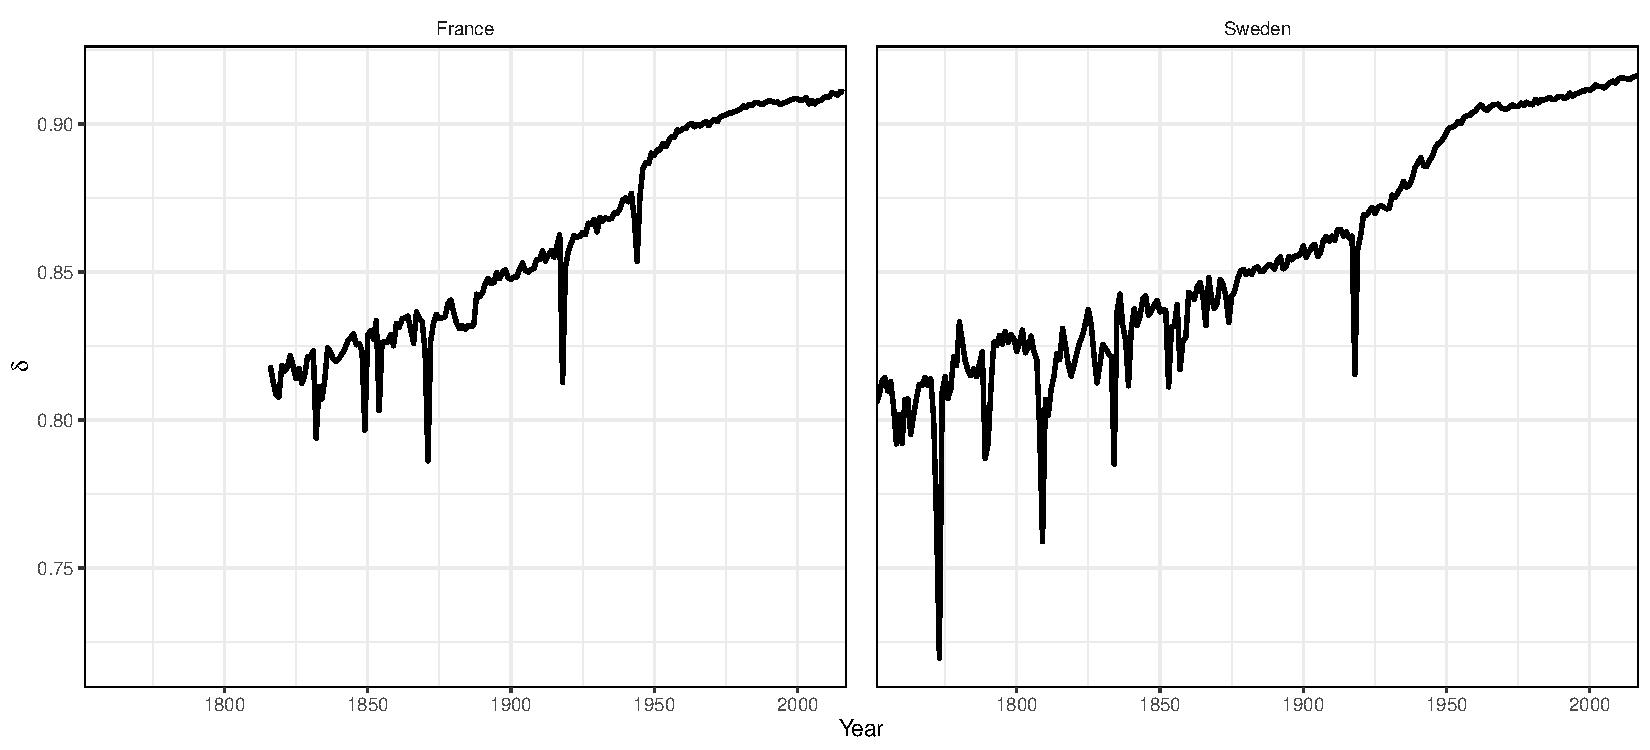
\includegraphics[scale=.6]{Figures/Figure_delta}
\label{Fig:delta}
\end{figure}


\end{document} 

